\documentclass[main.tex]{subfiles}
\begin{document}

\fixednote{Добре е тук да се направи кратко въведение в трета глава}

This section will discuss a practical implementation of an English-to-Overpass
translator, written as part of this thesis. The implementation contains a
parser for a custom language for defining CCGs, a CCG parser, an intermediate
language which can be easily generated via CCGs and translated into Overpass,
the respective translator and a web interface for evaluating queries.

\subsection{Architecture}
The system consists of several parts:

\cfigure{
    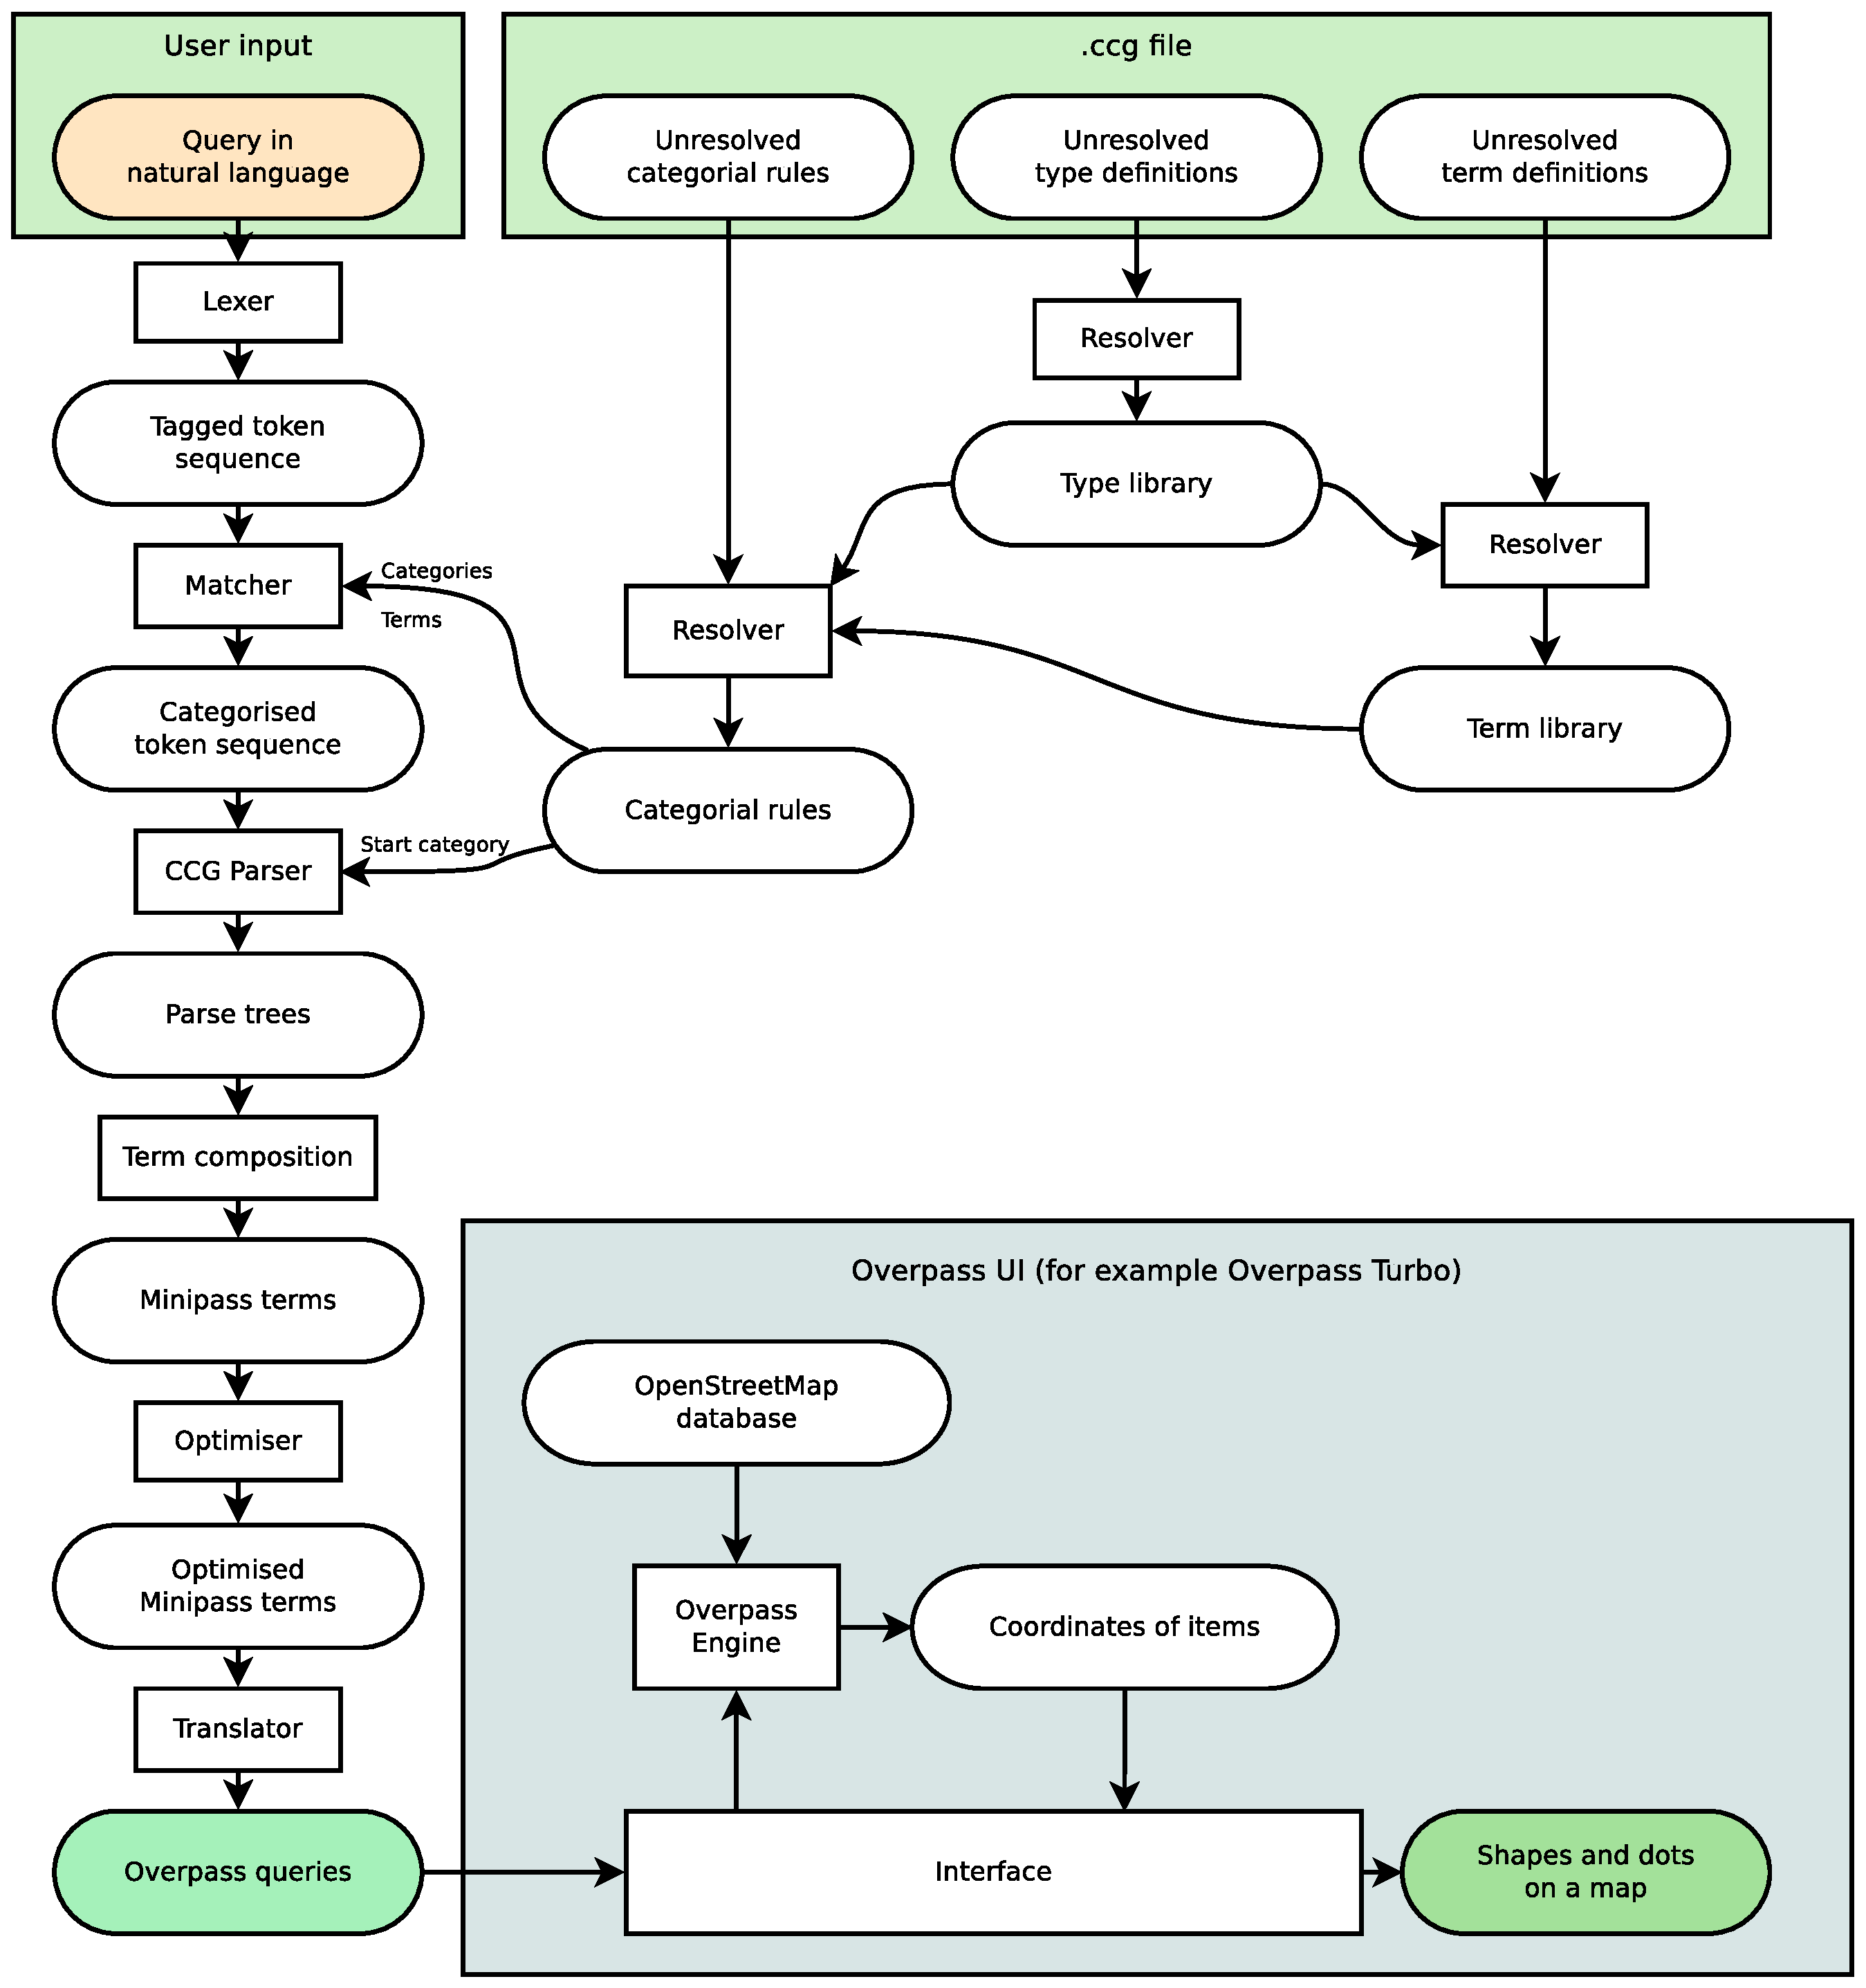
\includegraphics[width=\textwidth]{arch.eps}
    \caption{Architecture overview}
    \label{fig:arch}
}

\begin{itemize}
    \item Generic CCG definition language: a language for defining CCGs,
          their respective type systems and term libraries. Can be used
          standalone (for specifying CCGs that output raw parse trees)
          or by embedding a lambda calculus-based language (for specifying
          CCGs that output lambda terms)

    \item CCG Rule Matcher: a module that tags tokens from the input stream
          with categories based on the CCG rules (defined in the CCG definition
          language)

    \item CCG Parser: a simple proof-of-concept parser based on the CYK
          algorithm

    \item English Lexer: a tokeniser, POS-tagger, and lemmatiser for English
          (largely consists of external components)

    \item The Minipass language: a small, lambda calculus-based language
          that translates to Overpass, designed to be easily generated and
          to represent Overpass operators as operations on a graph.

    \item Minipass to Overpass translator: a translator from Minipass terms
          to Overpass queries that does some basic optimisations
\end{itemize}

An architecture overview can be seen at \cref{fig:arch}.

It is implemented in Haskell, and in addition to the query engine contains also
a demonstration web interface through which the user can enter a text query,
see the resulting Overpass query, inspect the intermediate steps (derivation
tree, minipass term before and after reduction) and finally view the results
on a map via Overpass Turbo (a public web interface for visualising queries
\cite{overpassturbo}).

An ``\emph{expert}'' can write grammar definitions that specify rules for matching
tokens and attaching categories and Minipass terms to them. This is done in
\code{.ccg} files, which can then be loaded at runtime and used for parsing the
input queries.

A sample grammar definition is provided, which can parse several sentence
constructions.

The pipeline can be easily modified to use a natural language other than
English, since the only language-dependent components are the tokeniser and
the grammar definition, which are straightforward to replace.
\end{document}
